\chapter{Iterative Methods}

\section{second order ODE's}

Most of FEM problems are \textbf{second order Ordinary Differential Equations}, e.g:

\begin{eqarray}
    m \frac{u''(t)}{d^2 t} + c \frac{u'(t)}{dt} + k u(t) &= 0\\
    m \ddot{u} + c \dot{u} + k u &= 0\\
    m a + c v + ku &= 0
\end{eqarray}

while the iterative methods are for \textbf{first order ODE's} only.
A \textbf{substitution} technique is therefore used to transform the
\textbf{second order ODE's} to a set of \textbf{first order ODE's} and these are
then solved sequentialy.

First we begin with a \textbf{second order ODE} in the form of:

\begin{equation}
    a \frac{y''(x)}{d^2 x} + b \frac{y'(x)}{dx} + c y = d, \quad with \quad y(0) = y_0 \quad and \quad
    \frac{y'(0)}{dx} = y_1
\end{equation}

By stating:

\begin{equation}
    \frac{dy}{dx} = z
\end{equation}

and substituting back:

\begin{equation}
    a \frac{dz}{dx} + b z + c y = d
\end{equation}

now we can write the following set of equations:

\begin{eqarray}
    \begin{aligned}
        z &= \frac{dy}{dx}\\
        \frac{dz}{dx} &= \frac{d - c y - b z}{a}
    \end{aligned} &
    \quad \left\{
    \begin{aligned}
        y(0) &= y_0\\
        z(0) &= y_1
    \end{aligned} \right.
\end{eqarray}



\section{Explicit}

\subsection{Euler's method}
The \textbf{Euler's Method} is an iterative method to solve ODEs. This method's
huge plus is it is fast. The minus is it gradually diverges from the ideal solution.

The \textbf{Euler's Method} uses the following formula:

\begin{equation}
    y(t + h) = y(t) + h f(x,y)
\end{equation}

to construct the tangent at point $ x $ and obtain the value of $ y(x + h) $,
whose slope is:

\begin{equation}
    f(x,y) \quad or \quad \frac{dy}{dx}
\end{equation}

\begin{figure}[ht]
    \centering
    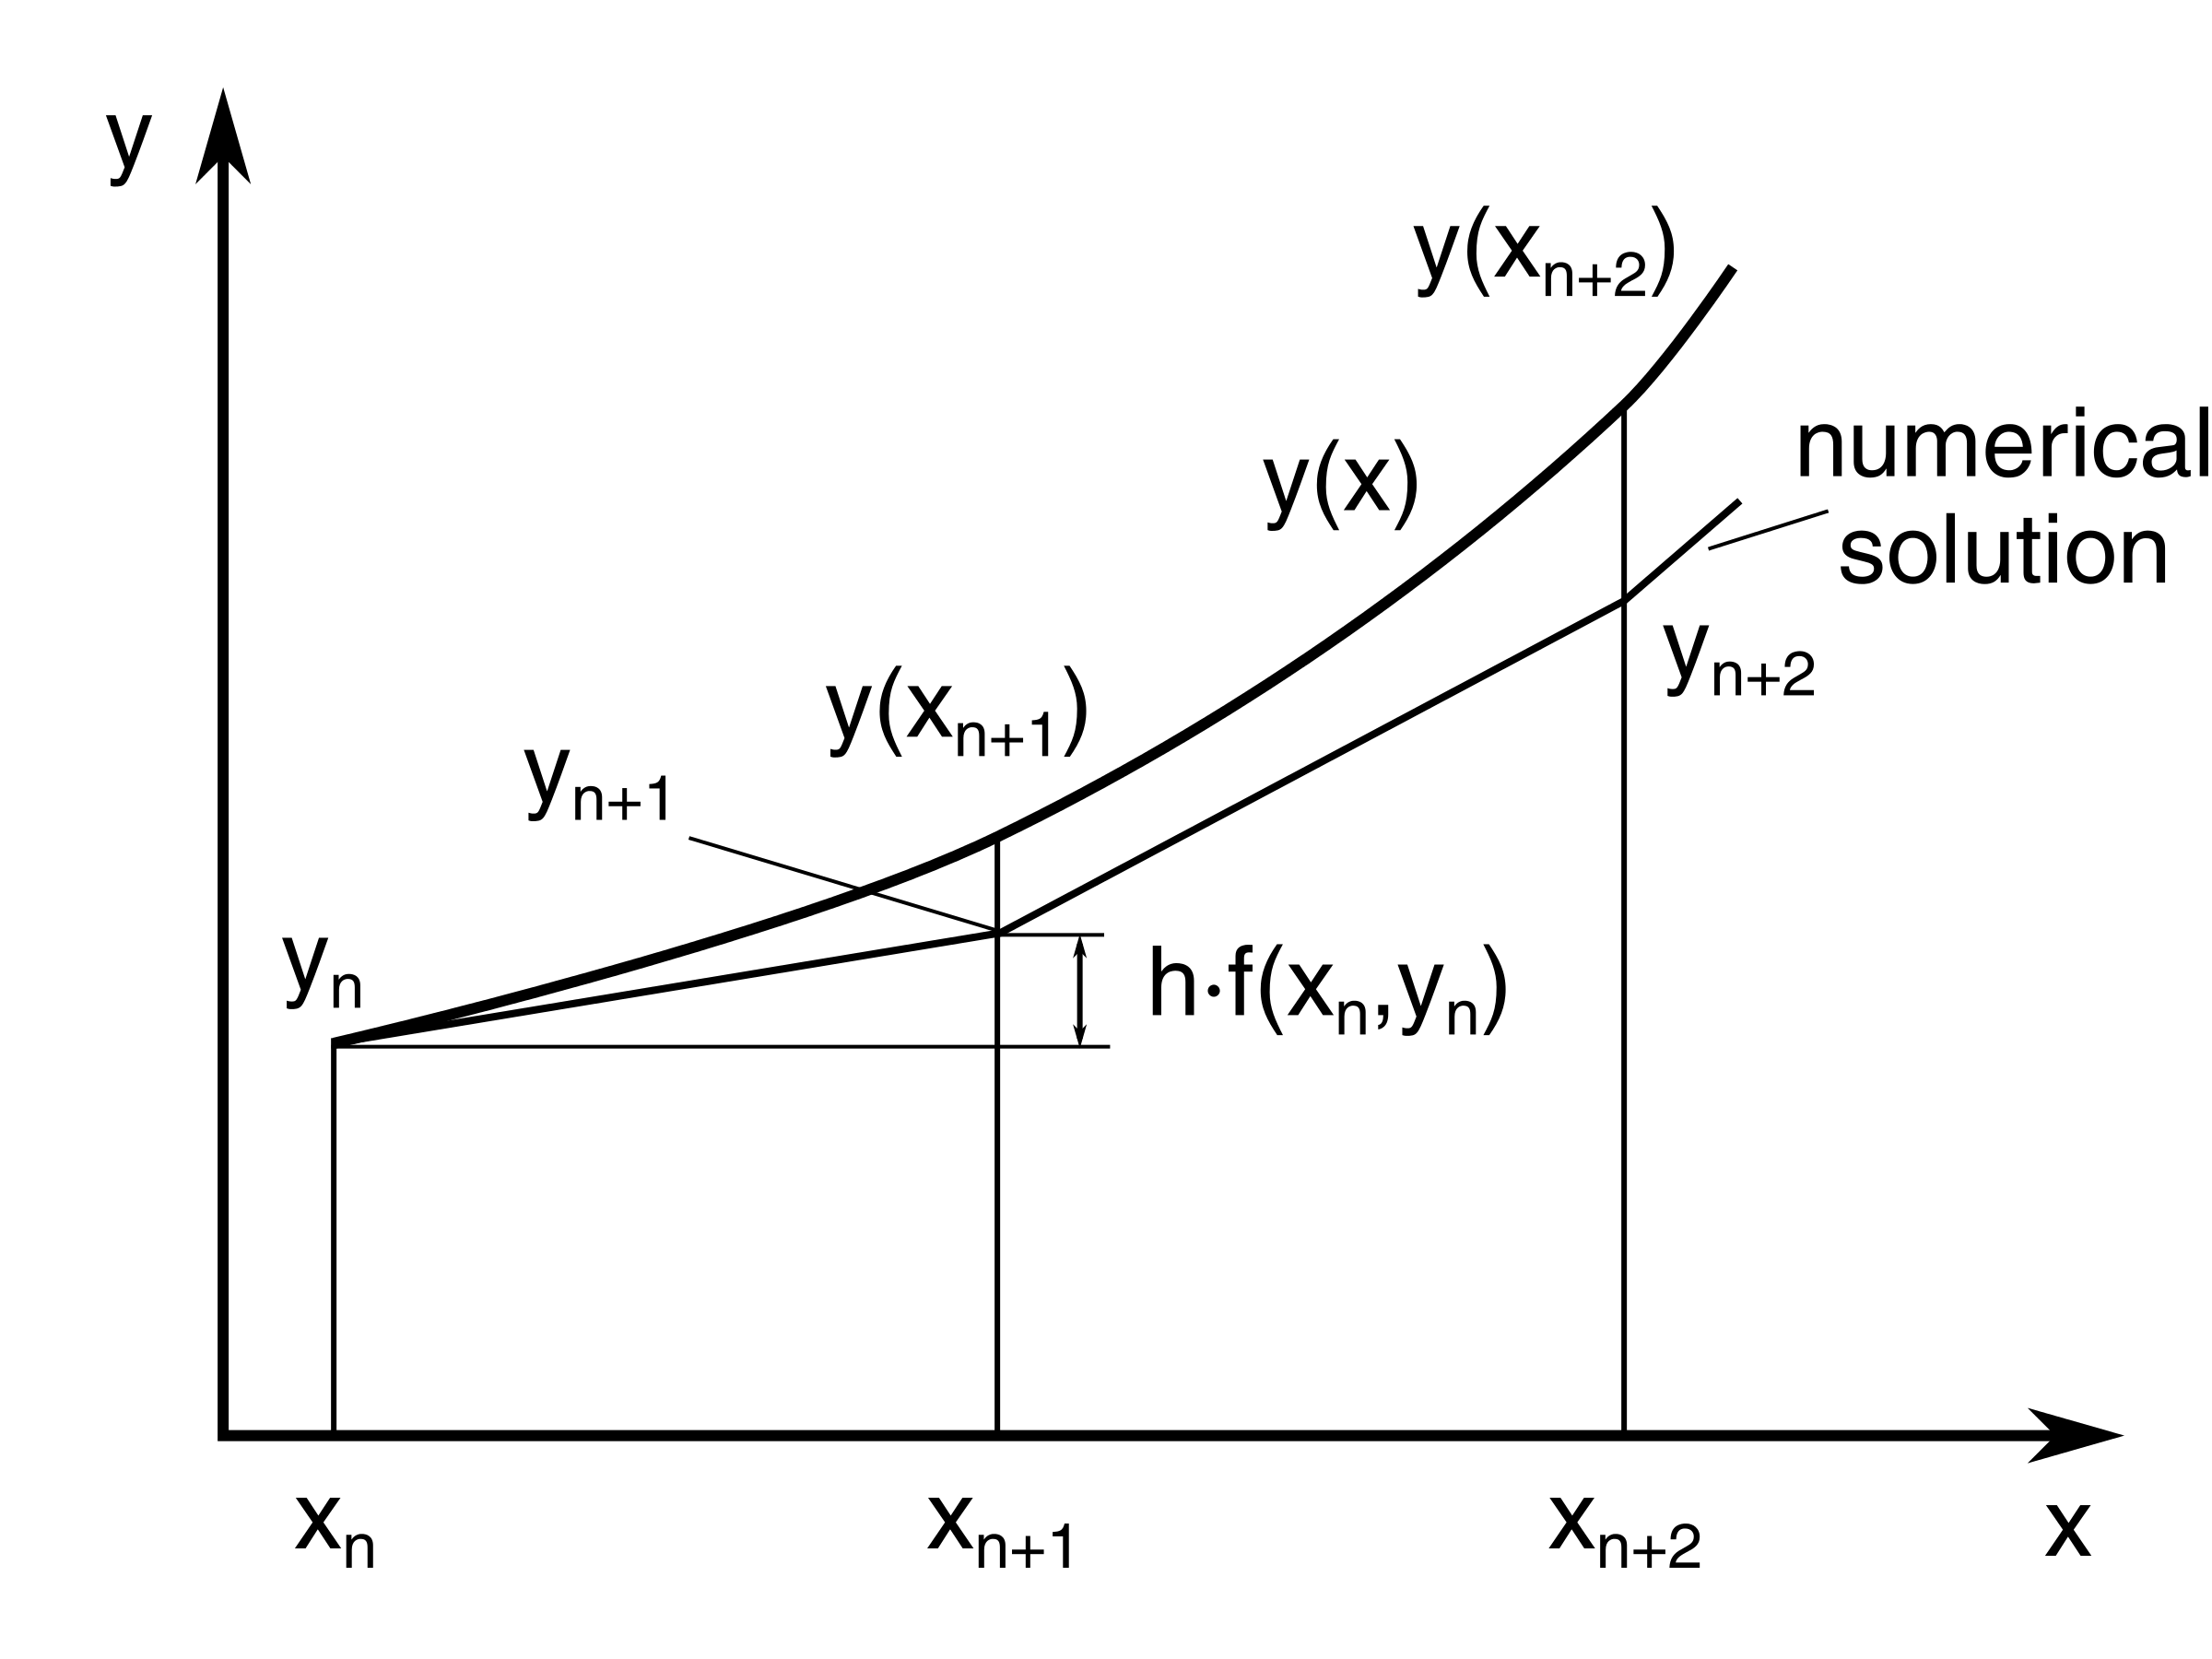
\includegraphics[width=0.90\textwidth]{img/Euler.png}
    \caption{Euler's method schematic}
    \label{fig:euler-png}
\end{figure}

In Euler's method, you can approximate the curve of the solution byt the tangent
in each interval (that is, by a sequence of shor line segments), at steps of $ h $.

\textit{In general}, if you use small step size, the accuracy of the approximation
increases.

\textbf{General Formula}

\begin{equation}
    y_{i+1} = y_i + h f(x_i,y_i)
\end{equation}

where:\\
$ y_{i+1} $ is the next estimated solution value,\\
$ y_i $ is the current value,\\
$ h $ is the interval between steps and\\
$ f(x_i,y_i) $ is the value of the derivative at the current $ (x_i,y_i) $ point.

\textbf{Pseudocode:}

\begin{itemize}
    \item define: $ f(x,y) $

    \item input: $ x_0 $, $ y_0 $

    \item input: $ h $, $ n $

    \item for $ j $ from $ 0 $ to $ (n-1) $ do
        \begin{itemize}
            \item $ y_{j+1} = y_j + hf(x_j, y_j) $
            \item $ x_{j+1} = x_j + h $
            \item Print $ x_{j+1} $ and $= y_{j+1} $
        \end{itemize}
    \item End.
\end{itemize}


\begin{bbox}[0.96]
\textbf{Note:}

If thinking about a problem in time domain:

\begin{itemize}
    \item define: $ f(t,x) $

    \item input: $ t_0 $, $ x_0 $

    \item input: $ dt $, $ n $

    \item for $ j $ from $ 0 $ to $ (n-1) $ do
        \begin{itemize}
            \item $ x_{j+1} = x_j + dt f(t_j, x_j) $
            \item $ t_{j+1} = t_j + dt $
            \item Print $ t_{j+1} $ and $= x_{j+1} $
        \end{itemize}
    \item end.
\end{itemize}

\end{bbox}


\newpage
\textbf{Python Code for vibration problem:}

\begin{python}
#!/usr/bin/python3
import numpy as np
import matplotlib.pyplot as plt


def iterate(h, y0, func, rhs):
    num_of_odes = y0.shape[0]
    y1 = np.zeros(num_of_odes, dtype = float)
    for i in range(num_of_odes-1):
        y1[i] = y0[i] + y0[i+1] * h
    y1[-1] = func(y1, rhs)
    return y1


def euler(t, y, func, rhs):
    N = t.shape[0]
    for j in range(N-1):
        dt = t[j+1] - t[j]
        y[j+1,:] = iterate(dt, y[j,:], func, rhs[j])
        # print(y[j+1,:])
    return y


def euler_vibration():
    m = 0.55  # tonnes
    c = 3.    # Ns/mm
    k = 1000. # N/mm

    freq = np.sqrt(k / m) / (2 * np.pi)

    # equation to solve
    # m * a + c * v + k * u = f
    # a = (f - c * v - k * u) / m
    acceleration = lambda u, f: (f - c * u[1] - k * u[0]) / m

    T = 2.0     # seconds
    dt = 0.0001 # timestep s
    u_0 = 0.    # mm of initial displacement
    v_0 = 0.    # mm/s of initial velocity

    # times at which to solve
    t = np.linspace(0, T, int(T/dt) + 1)

    # force vector
    F = 5000. # N of max impulse
    t0 = 0.1  # impulse start time
    t1 = 0.2  # impuls end time
    f = np.zeros(t.shape[0], dtype=float)
    # create a half sine impulse of force
    for i in range(t.shape[0]):
        if t[i] >= t0 and t[i] <= t1:
            f[i] = F * np.sin((t[i] - t0) / (t1 - t0) * np.pi)
        else:
            f[i] = 0.

    uva = np.zeros((t.shape[0],3), dtype=float)
    uva[0,0] = u_0
    uva[0,1] = v_0

    uva = euler(t, uva, acceleration, f)

    fig, axf = plt.subplots()
    fig.subplots_adjust(right=0.60)

    p1, = axf.plot(t, f, label='force', color='violet')
    axu = axf.twinx()
    p2, = axu.plot(t, uva[:,0], label='displacement', color='red')
    axv = axf.twinx()
    axv.spines.right.set_position(('axes', 1.20))
    p3, = axv.plot(t, uva[:,1], label='velocity', color='blue')
    axa = axf.twinx()
    axa.spines.right.set_position(('axes', 1.40))
    p4, = axa.plot(t, uva[:,2], label='acceleration', color='green')

    axf.set_xlabel('Time [s]')
    axf.set_ylabel('Force [N]')
    axu.set_ylabel('Displacement [mm]')
    axv.set_ylabel('Velocity [mm/s]')
    axa.set_ylabel('Acceleration [mm/s2]')

    axf.legend(handles=[p1, p2, p3, p4])

    plt.show()

if __name__ == '__main__':
    euler_vibration()

\end{python}

Which results to:
\begin{figure}[ht]
    \centering
    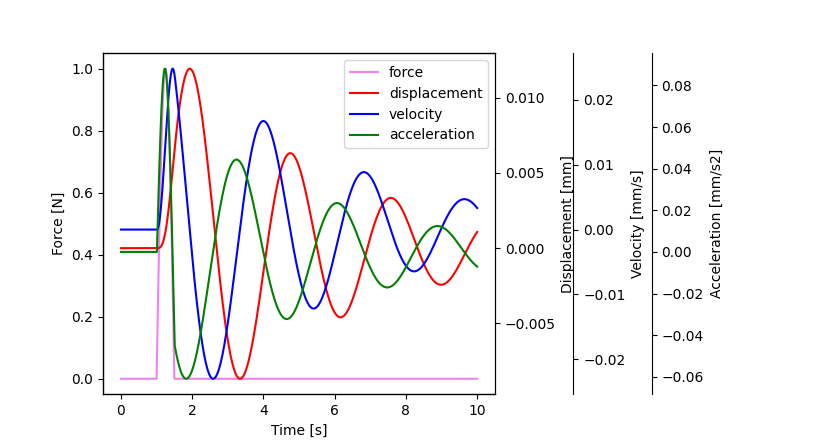
\includegraphics[width=0.90\textwidth]{img/euler_example.png}
    \caption{Euler's implementation for vibration problem example}
    \label{fig:euler-example-png}
\end{figure}


The \textbf{iterate()} function:
\begin{python}
def iterate(h, y0, func, rhs):
    num_of_odes = y0.shape[0]
    y1 = np.zeros(num_of_odes, dtype = float)
    for i in range(num_of_odes-1):
        y1[i] = y0[i] + y0[i+1] * h
    y1[-1] = func(y1, rhs)
    return y1

\end{python}

is written for general case of a set of ODEs. When considering the problem
of vibration (set of 2 ODEs):
\begin{python}
def iterate(h, u0, v0, a0, f, m , c, k):
    u1 = u0 + h * v0
    v1 = v0 + h * a0
    # m * a + c * v + k * u = f
    a1 = (f - c * v1 - k * u1) / m
    return np.array([u1, v1, a1], dtype=float)
\end{python}

which is the iteration of a set of \textbf{first order ODEs}:
\begin{eqarray}
    v &= \dot{u}\\
    \dot{v} &= \frac{f - c * v - k * u}{m}
\end{eqarray}


\newpage
\subsection{Runge-Kutta 4th order method}

\textbf{Runge-Kutta 4th order method} is another explicit method for solving
\textbf{first order ODEs}. The basic equation is:

\begin{equation}
    \frac{dy}{dx} = f(x,y) \quad , y(0) = y_0
\end{equation}

The formula for the next value $ y_{i+1} $ after a step size equal to $h $ is given by:

\begin{eqarray}
    k_1 &= h f(x_i, y_i)\\
    k_2 &= h f(x_i + \frac{h}{2}, y_i + \frac{k_1}{2})\\
    k_3 &= h f(x_i + \frac{h}{2}, y_i + \frac{k_2}{2})\\
    k_4 &= h f(x_i + h, y_i + k_3)\\
    y_{i+1} &= y_i + \frac{k_1}{6} + \frac{k_2}{3} + \frac{k_3}{3} + \frac{k_4}{6} + O(h^5)
\end{eqarray}

The formula basically computes next value $ y_{i+1} $ using current $ y_i $ plus
\textbf{weighted average of four increments}:

\begin{itemize}
    \item $ k_1 $ is the increment based on the slope at the beginning of the
    interval, using $ y $

    \item $ k_2 $ is the increment based on the slope at the midpoint of the interval,
        using $ y + h k_1 / 2 $

    \item $ k_3 $ is the increment based on the slope at the midpoint,
        using $ y + h k_2 / 2 $

    \item $ k_4 $ is the increment based on the slope at the end of the interval,
        using $ y + h k_3 / 2 $

\end{itemize}

The method is a fourth order method, meaning that the local truncation error is
on the order of $ O(h^5) $, while the total accumulated error is of order $ O(h^4) $.

\begin{figure}[ht]
    \centering
    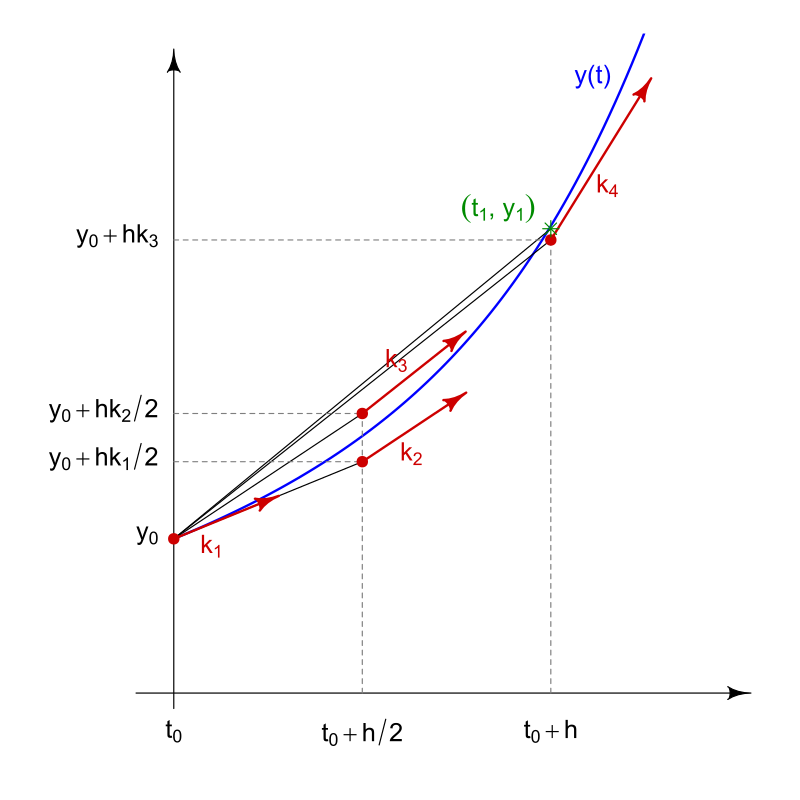
\includegraphics[width=0.80\textwidth]{img/Runge-Kutta_slopes.png}
    \caption{4th Order Runge-Kutta's method schematic}
    \label{fig:rk4-schema-png}
\end{figure}

\newpage
\begin{bbox}[0.96]
\textbf{Note:}

The formula for the next value $ y_{i+1} $ can be also written as:

\begin{eqarray}
    k_1 &= y_i\\
    k_2 &= y_i + \frac{h}{2} \frac{d k_1}{dx}\\
    k_3 &= y_i + \frac{h}{2} \frac{d k_2}{dx}\\
    k_4 &= y_i + h \frac{k_3}{dx}\\
    y_{i+1} &= y_i + \frac{h}{6} (\frac{d k_1}{dx} + 2 \frac{d k_2}{dx}
                              + 2 \frac{d k_3}{dx} + \frac{d k_4}{dx}) + O(h^5)
\end{eqarray}
\end{bbox}

\begin{bbox}[0.96]
This notation is more convenient to use when solving sets of ODEs for vibration
problem, because it translates to:

\begin{eqarray}
    u_1 &= u_0\\
    v_1 &= v_0\\
    a_1 &= (f - c v_0 - k u_0) / m\\
    u_2 &= u_0 + \frac{h}{2} v_1\\
    v_2 &= v_0 + \frac{h}{2} a_1\\
    a_2 &= (f - c v_1 - k u_1) / m\\
    u_3 &= u_0 + \frac{h}{2} v_2\\
    v_3 &= v_0 + \frac{h}{2} a_2\\
    a_3 &= (f - c v_2 - k u_2) / m\\
    u_4 &= u_0 + h v_3\\
    v_4 &= v_0 + h a_3\\
    a_4 &= (f - c v_3 - k u_3) / m\\
    u_{i+1} &= u_0 + \frac{h}{6} \left( v_1 + 2 v_2 + 2 v_3 + v_4 \right) \\
    v_{i+1} &= v_0 + \frac{h}{6} \left( a_1 + 2 a_2 + 2 a_3 + a_4 \right) \\
    a_{i+1} &= (f - c v_{i+1} - k u_{i+1}) / m\\
\end{eqarray}

where each of the \textbf{ODEs} are solved sequentially from the values
already known.

\end{bbox}

\newpage
\textbf{Python implementation for vibration problem:}

\begin{python}
#!/usr/bin/python3
import numpy as np
import matplotlib.pyplot as plt


def iterate(h, y0, y, func, rhs):
    num_of_odes = y0.shape[0]
    y1 = np.zeros(num_of_odes, dtype = float)
    for i in range(num_of_odes-1):
        y1[i] = y0[i] + y[i+1] * h
    y1[-1] = func(y1, rhs)
    return y1


def runge_kutta_4(t, y, func, rhs):
    N = t.shape[0]
    for j in range(N-1):
        dt = t[j+1] - t[j]
        y1 = iterate(0., y[j,:], y[j,:], func, rhs[j])
        y2 = iterate(dt/2, y[j,:], y1, func, 0.5 * (rhs[j+1] + rhs[j]))
        y3 = iterate(dt/2, y[j,:], y2, func, 0.5 * (rhs[j+1] + rhs[j]))
        y4 = iterate(dt, y[j,:], y3, func, rhs[j+1])

        # next step solution
        for i in range(y.shape[1]-1):
            y[j+1,i] = y[j,i] + dt/6 * (y1[i+1] + 2 * y2[i+1] + 2 * y3[i+1] + y4[i+1])
        y[j+1,-1] = func(y[j+1,:], rhs[j+1])
    return y


def rk4_vibration():
    m = 10.   # tonnes
    c = 5.    # Ns/mm
    k = 50.   # N/mm

    freq = np.sqrt(k / m) / (2 * np.pi)
    print(f'f = {freq}')

    # equation to solve
    # m * a + c * v + k * u = f
    # a = (f - c * v - k * u) / m
    acceleration = lambda u, f: (f - c * u[1] - k * u[0]) / m

    T = 10.     # seconds
    dt = 0.01   # timestep s
    u_0 = 0.    # mm of initial displacement
    v_0 = 0.    # mm/s of initial velocity

    # times at which to solve
    t = np.linspace(0, T, int(T/dt) + 1)

    # force vector
    F = 1.    # N of max impulse
    t0 = 1.   # impulse start time
    t1 = 1.5  # impuls end time
    f = np.zeros(t.shape[0], dtype=float)
    # create a half sine impulse of force
    for i in range(t.shape[0]):
        if t[i] >= t0 and t[i] <= t1:
            f[i] = F * np.sin((t[i] - t0) / (t1 - t0) * np.pi)
        else:
            f[i] = 0.

    uva = np.zeros((t.shape[0],3), dtype=float)
    uva[0,0] = u_0
    uva[0,1] = v_0

    uva = runge_kutta_4(t, uva, acceleration, f)

    fig, axf = plt.subplots()
    fig.subplots_adjust(right=0.60)

    p1, = axf.plot(t, f, label='force', color='violet')
    axu = axf.twinx()
    p2, = axu.plot(t, uva[:,0], label='displacement', color='red')
    axv = axf.twinx()
    axv.spines.right.set_position(('axes', 1.20))
    p3, = axv.plot(t, uva[:,1], label='velocity', color='blue')
    axa = axf.twinx()
    axa.spines.right.set_position(('axes', 1.40))
    p4, = axa.plot(t, uva[:,2], label='acceleration', color='green')

    axf.set_xlabel('Time [s]')
    axf.set_ylabel('Force [N]')
    axu.set_ylabel('Displacement [mm]')
    axv.set_ylabel('Velocity [mm/s]')
    axa.set_ylabel('Acceleration [mm/s2]')

    axf.legend(handles=[p1, p2, p3, p4])

    plt.show()

if __name__ == '__main__':
    rk4_vibration()

\end{python}

Which results to:
\begin{figure}[ht]
    \centering
    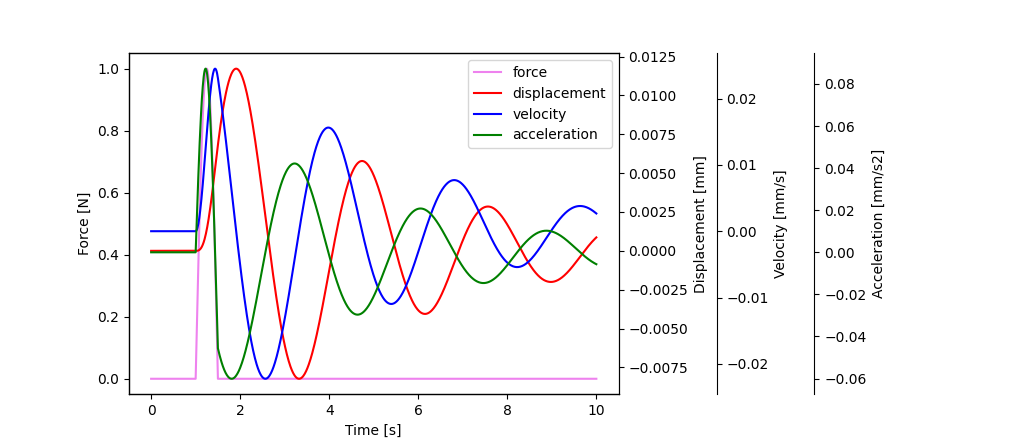
\includegraphics[width=0.90\textwidth]{img/rk4_example.png}
    \caption{4th order Runge-Kutta's implementation for vibration problem example}
    \label{fig:rk4-example-png}
\end{figure}



\newpage
\section{Implicit}

The basic approach is an incremental step-by-step solution with an assumtion
that the solution for a discrete time $ t $ is known and that the solution for
the discrete time $ t + \Delta t $ is required, where $ \Delta t $ is
a suitably chosen time increment. Hence, considering time $ t + \Delta t $:

\begin{equation}\label{implicit-equation}
    \m{F}^{t + \Delta t} - \m{N}^{t + \Delta t} = \m{0}
\end{equation}

Where $ \m{F} $ is the vector of external forces (loads) and $ \m{N} $
is the vector of inner forces.

Assume that $ \m{F}^{t + \Delta t} $ is independent of the deformations.
Since the solution is known at time $ t $, we can write:

\begin{equation}
    \m{N}^{t+\Delta t} = \m{N}^t + \Delta \m{N}
\end{equation}

where $ \Delta \m{N} $ is the increment in nodal point forces corresponding
to the increment in element displacements and stresses from time $ t $ to time
$ t + \Delta t $. This vector can be approximated using a \textbf{tangent stiffness matrix}
$ \m{K}^t $ which corresponds to the geometric and material conditions
at time $ t $,

\begin{equation}\label{internal-forces-approximation}
    \Delta \m{N} \doteq \m{K}^{t} \Delta \m{u}
\end{equation}

where $ \Delta \m{u} $ is a vector of incremental nodal point displacements and

\begin{equation}\label{tangent-stiffness-matrix}
    \m{K}^{t} = \frac{\partial \m{N}^{t}}{\partial \m{u}^{t}}
\end{equation}

Hence, the \textbf{tangent stiffness matrix} corresponds to the derivative of the
internal element nodal point forces $ \m{N}^{t} $ with respect to the
nodal point displacements $ \m{u}^{t} $.

Substituting \eqref{internal-forces-approximation} and
\eqref{tangent-stiffness-matrix} into \eqref{implicit-equation}, we obtain

\begin{equation}\label{iteration-equation}
    \m{K}^{t} \Delta \m{u} = \m{F}^{t + \Delta t} - \m{N}^{t}
\end{equation}

and solving for $ \m{u}^{\Delta t} $, we can calculate and approximation
to the displacements at time $ t + \Delta t $,

\begin{equation}\label{iteration-displacements}
    \m{u}^{t + \Delta t} \doteq \m{u}^{t} + \Delta \m{u}
\end{equation}

The exact displacements at time $ t + \Delta t $ are those that correspond to the
applied loads $ \m{F}^{t + \Delta t} $. We calculate in \eqref{iteration-displacements}
only an approximation to these displacements because \eqref{internal-forces-approximation}
was used.

Having evaluated an approximation to the displacements corresponding to
time $ t + \Delta t $, we could now solve for an approximation to the stresses and
corresponding nodal point forces at time $ t + \Delta t $, and then proceed to the
next time increment calculations. However, because of the assumption
\eqref{internal-forces-approximation}, such a solution may be subject to
very significant errors and, depending on the time or load step sizes used, may
indeed be unstable. In practice, it is therefore necessary to iterate until the
solution of \eqref{implicit-equation} is obtained to sufficient accuracy.


\subsection{Newton-Raphson}
Having calculated an \textit{increment} in nodal point displacements, which defones
a \textit{new total} displacement vector, we can repeat ht incremental solution
using the currently known total displacements at time $ t $.

The equations used in \textbf{Newton-Raphson} iteration are, $ for\ i = 1, 2, 3, \dots, $

\begin{bbox}
    \begin{eqarray}\label{newton-raphson}
        \m{K}_{i-1}^{t + \Delta t} \Delta \m{u}_i &=
        \m{F}^{t + \Delta t} - \m{N}_{i - 1}^{t + \Delta t} \\
        \m{u}_{i}^{t+\Delta t} &=  \m{u}_{i}^{t + \Delta t} +
        \m{u}_{i-1}^{t+\Delta t} + \Delta \m{u}_i
    \end{eqarray}
\end{bbox}

with the initial conditions:

\begin{eqarray}
    \m{u}_{0}^{t + \Delta t} &= \m{u}^t \\
    \m{K}_{0}^{t + \Delta t} &= \m{K}^t \\
    \m{N}_{0}^{t + \Delta t} &= \m{N}^t \\
\end{eqarray}

Note that in the first iteration, the relations in \eqref{newton-raphson}
reduce to the equations \eqref{iteration-equation} and \eqref{iteration-displacements}.
Then, in subsequent iterations, the latest estimates for the nodal point
displacements are used to evaluate the corresponding element stresses and
nodal point forces $ \m{N}_{i-1}^{t + \Delta t} $ and
\textbf{tangent stiffness matrix} $ \m{K}_{i-1}^{t + \Delta t} $.

The out-of-balance load vector $ \m{F}^{t + \Delta t} - \m{N}_{i-1}^{t + \Delta t} $
corresponds to a load vector that is not yet balanced by element stress, and
hence an increment in the nodal point displacement is required. This updating of the
nodal point displacement in the iteration is continued until out-of-balance loads
and incremental displacements are small enough.

An important point is that the calculation of $ \m{N}_{i-1}^{t + \Delta t} $
from $ \m{u}_{i-1}^{t + \Delta t} $ is \textbf{crucial}. Any errors in this
calculation will, in general, result in an incorrect response prediction.

The correct evaluation of the \textbf{tangent stiffness matrix}
$ \m{K}_{i-1}^{t + \Delta t} $ is also important. The use of proper
\textbf{tangent stiffness matrix} may be necessary for convergence and, in general,
will result in fewer iterations until convergence is reached.

However, because the expense involved in evaluating and factoring a new
\textbf{tangent stiffness matrix}, in practice, it can be more efficient,
depending on the nonlinearities present in the analysis, to evaluate a new
\textbf{tangent stiffness matrix} only at certain times. Specifically,
in the \textbf{modified Newton-Raphson method} a new \textbf{tangent stiffness matrix}
is established only at the beginning of each load step, and in
\textbf{quasi-Newton} methods \textbf{secant stiffness matrices} are used
instead of the tangent stiffness matrix.

The use of the iterative solution requires appropriate convergence criteria.
If inappropriate criteria are used, the iteration may be terminated before
the necessary solution accuracy is reached or be continued after the required
accuracy has been reached.

\subsubsection{Full Newton-Raphson Procedure derivation}

The finite element equilibrium requirements amount to finding the solution
of the equations:

\begin{equation}\label{nr-error}
    f( \m{u}^* ) = 0
\end{equation}

Where:

\begin{equation}\label{nr-error-expanded}
    f( \m{u}^* ) = \m{F}^{t + \Delta t} ( \m{u}^* )
    - \m{N}^{t + \Delta t} ( \m{u}^* )
\end{equation}

We denote here and in the following the complete array of the solution as
$ \m{u}^* $ but realize that this vector may also contain variables other
than displacements, for example, pressure variables and rotations.

Assume that in the iterative solution we have evaluated $ \m{u}_{i-1}^{t + \Delta t} $;
then a Taylor series expansion gives:

\begin{eqarray}\label{newton-raphson-taylor-expansion}
    f(\m{u}^*) &= f(\m{u}_{i-1}^{t + \Delta t})
    + \left. \left[\frac{\partial N}{\partial \m{u}} \right]
        \right|_{\m{u}_{i-1}^{t + \Delta t}}
        \left( \m{u}^* - \m{u}_{i-1}^{t + \Delta t} \right) \\
                    &+ higher\ order\ terms
\end{eqarray}

Substituting from \eqref{nr-error-expanded} into \eqref{newton-raphson-taylor-expansion}
and using \eqref{nr-error}, we obtain:

\begin{eqarray}\label{nr-taylor}
    & \left. \left[ \frac{\partial \m{N}}{\partial \m{u}} \right]
        \right|_{\m{u}_{i-1}^{t + \Delta t}}
    \left(\m{u}^* - \m{u}_{i-1}^{t + \Delta t} \right)
    + higher\ order\ terms\\
    & = \m{F}^{t + \Delta t} - \m{N}_{i-1}^{t + \Delta t}
\end{eqarray}

where we assumed that the externally applied loads are deformation independent.

Neglecting the higher-order terms in \eqref{nr-taylor}, we can calculate an increment
in the displacements,

\begin{equation}\label{nr-displacement-increment}
    \m{K}_{i-1}^{t + \Delta t} \Delta \m{u}_i =
    \m{F}^{t + \Delta t} - \m{N}_{i-1}^{t + \Delta t}
\end{equation}

where $ \m{K}_{i-1}^{t + \Delta t} $ is the current \textbf{tangent stiffness matrix}

\begin{equation}
     \m{K}_{i-1}^{t + \Delta t} =
     \left. \left[ \frac{\partial \m{N}}{\partial \m{u}} \right]
        \right|_{\m{u}_{i-1}^{t + \Delta t}}
\end{equation}

and the improved displacement solution is:

\begin{equation}\label{nr-displacement}
    \m{u}_i^{t + \Delta t} =
    \m{u}_{i-1}^{t + \Delta t} +
    \Delta \m{u}_{i}
\end{equation}

\textit{The relations in} \eqref{nr-displacement-increment} \textit{and} \eqref{nr-displacement}
\textit{costitute the Newton-Raphson solution of} \eqref{implicit-equation}.
Since an incremental analysis is performed with time (or load) steps of size
$ \Delta t $, the initial conditions in this iteration are
$ \m{K}_0^{t + \Delta t} = \m{K}^t $,
$ \m{N}_0^{t + \Delta t} = \m{N}^t $, and
$ \m{u}_0^{t + \Delta t} = \m{u}^t $.
The iteration is continued \textbf{until appropriate convergence criteria are satisfied.}

A characteristic of this iteration is that a new tangent stiffness matrix is
calculated in \textbf{each} iteration, which is why this method is also referred
to as the \textbf{full Newton-Raphson method}.

\begin{figure}[ht]
    \centering
    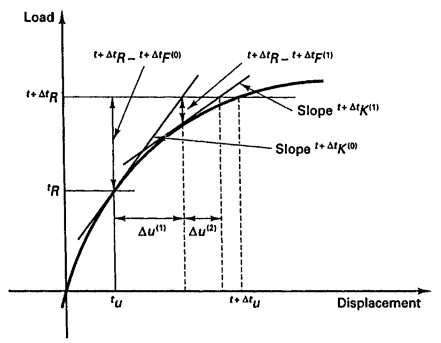
\includegraphics[width=0.60\textwidth]{img/full_newton_raphson.png}
    \caption{Newton-Raphson iteration in solution of SDOF system.
    $ \m{R} $ is load increment, $ \m{F} $ are internal forces,
    $ \m{u} $ are displacements.}
    \label{fig:full-newton-raphson-png}
\end{figure}

% TODO: Bathe FEP_2nd_Edidtion_4th_prinitng.pdf
%       Page 756 (773)
%       Modified Newton-Raphson

